\documentclass{standalone}
\usepackage{pgfplots}
\pgfplotsset{compat=1.11}
\begin{document}
% Place the TikZ picture in a figure environment.
%\begin{figure}[htb]
% h: here, t: top, b: bottom, p: page of float
%% https://tex.stackexchange.com/questions/39017/how-to-influence-the-position-of-float-environments-like-figure-and-table-in-lat
%% ! indicates that some restrictions should be ignored (discussed later)
%% h indicates that the float is allowed to be placed inline
%% t indicates that the float is allowed to go into a top area
%% b indicates that the float is allowed to go into a bottom area
%% p indicates the the float is allowed to go on a float page or column area

    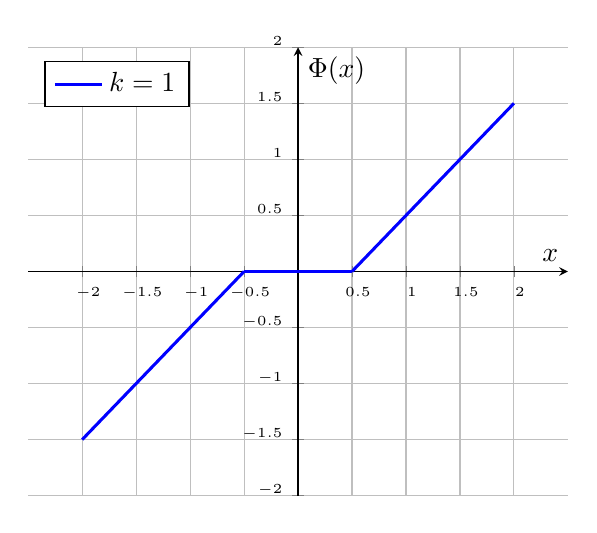
\begin{tikzpicture}
        \begin{axis} [
            xmin=-2.5, xmax=2.5, ymin=-2, ymax=2, grid=both,
            ylabel={$\Phi(x)$}, xlabel={$x$},
            xtick={-2,-1.5,...,2}, ytick={-2,-1.5,...,2},
            xticklabel style={font=\tiny, xshift=0.5ex},
            yticklabel style={font=\tiny, yshift=0.5ex},
            axis line style={->},
            axis x line=middle,
            axis y line=middle,
            legend pos=north west,
        ]
        \addplot+[mark=none, line width=1.1, color=blue, domain=-2:-0.5] {x+0.5};
        \addplot+[mark=none, line width=1.1, color=blue, domain=-0.5:0.5] {0};
        \addplot+[mark=none, line width=1.1, color=blue, domain=0.5:2] {x-0.5};
        \addlegendentry{$k=1$}
        \end{axis}
    \end{tikzpicture}

\end{document}